% BEÁLLÍTÁSOK - JOBB NEM VÁLTOZTATNI
\documentclass[final]{ubb_dolgozat}
\usepackage{definitions}
\usepackage{wrapfig}
\usepackage{color}


% milyen nyelveken akarunk forráskódot megjeleníteni
\lstloadlanguages{Java,C++}
% más lehetőségek:
% C, Matlab, Mathematica, Octave, Pascal, Perl, Python
% SCilab, SQL, Haskell, Lisp, Lua, make, ML, PHP, Prolog
%
% a teljes lista a LISTINGS csomagban.


% ezt be lehet tenni MINDEGYIK megjelenítendő kód elé opcióként
\lstset{language=Java}


%%%%%%%%%%%%%%%%%%%%%%%%%%%%%%%%%%%%%%%%%%%%%%%
%%!!          EZT KELL VÁLTOZTATNI       !!%%%%
%%     A DOLGOZAT CÍMOLDALÁNAK ELEMEI        %%

%% MELYIK ÉVBEN ADJUK LE
\submityear{%
2018
}

\titleHU{%
GRoutes - Az utazó ügynök problémájának gyakorlati alkalmazása
}

% Az alábbi sorokat ki kell tölteni!!

\titleEN{%
GRoutes - A practical application of the travelling salesman problem
}

\titleRO{%
GRoutes - O aplicație practică pentru problema comis-voiajorului
}

\author{%
Lorenzovici Zsombor
}

%%
\tutorHU{%
dr. Gaskó Noémi,\newline egyetemi docens\\
% a hozzátartozás akkor szükség, ha NEM BBTE-s a tanár
%{\large Babe\c{s}--Bolyai Tudományegyetem,\\
% Matematika és Informatika Kar}% ha különbözik, akkor fel kell tûntetni
}
%%
\tutorRO{%
Conf. dr. Gaskó Noémi\\
% az egyetem akkor szükség, ha nem BBTE-s a tanás, a minta a BBTE-t
% tartalmazza
% {\large Universitatea Babe\c{s}--Bolyai,\\ % dacã diferã!!!
% Facultatea de Matematic\u{a} \c{s}i Informatic\u{a} }%
}
%%
\tutorEN{%
Assoc. prof. dr. Gaskó Noémi
% {\large Babe\c{s}--Bolyai University,\\
% Faculty of Mathematics and Informatics}
}


% 
%\includeonly{bevezet}


\begin{document}

%% ABSTRAKT
\begin{abstractEN} % ANGOL VÁLTOZAT

% a lenti részt értelemszerûen ki kell tölteni a dolgozat angol kivonatával.
% A BEGIN ... END között CSAK A SAJÁT SZÖVEG kell, hogy legyen.
% Az utolsó mondatot benne kell hagyni, mely által kijelentitek, hogy a munkátok SAJÁT.

The present paper describes a practical application of the travelling salesman problem (TSP). In the first chapters I describe the theoretical background of the work, the definition of graphs, notions in graph theory, graph problems, algorithmic approaches, TSP algorithms, reduction of the asymmetric TSP to a symmetric one. The emphasis is on selecting an algorithm that matches, and serves our use case practically.

To exemplify the travelling salesman problem, I have developed an android application, with a Firestore database, Firebase Authentication and Maps API. The functionalities of the application include searching for locations, determining the best route (visiting every node), choosing the travelling mode (by car, on foot), automatically adapting the search algorithm, saving the searches, managing routes and places as favourites.

This work is the result of my own activity. I have neither given nor received unauthorized assistance on this work.

\end{abstractEN}

% ez a címoldal része
\maketitle

%% 

% a dolgozat tartalomjegyzéke -- ez automatikusan generálódik a STRUKTÚRA alapján.
{ \baselineskip 1ex
  \parskip 1ex
  \tableofcontents
}


%%%%%%%%%%%%%%%%%%%%%%%%%%%%%%%%%%%%%%%%%%%%%%%%%%%%%%%%%%%
%%%%%%%%%%         a dolgozat tartalma         %%%%%%%%%%%%

% ajánlott külön file-okba írni az egyes fejezeteket,
% ugyanis úgy jobban át lehet látni.


% a bevezetõ fejezet FILE-ja.
%!TEX root = GRoutes.tex
%%%%%%%%%%%%%%%%%%%%%%%%%%%%%%%%%%%%%%%%%%%%%%%%%%%%%%%%%%%%%%%%%%%%%%%
\chapter{Bevezetés}\label{ch:ALAP}
%%%%%%%%%%%%%%%%%%%%%%%%%%%%%%%%%%%%%%%%%%%%%%%%%%%%%%%%%%%%%%%%%%%%%%%

Dolgozatom témája az "utazó ügynök" problémájának (TSP)%
\footnote{ %
	Travelling salesman problem
}  %
 a gyakorlatban történő alkalmazása. Az utazó ügynök problémája egy komputacionális optimalizálási probléma, amely az 1930-as évek óta nagyon intenzíven foglalkoztatja a tudományos világot. Egyszerűen megfogalmazva: adott valamennyi város, valamint az köztük levő távolságok. Melyik a legrövidebb lehetséges útvonal, ami egyszer érinti az összes várost, majd visszaérkezik a kiinduló pontba? Jelenleg nem létezik olyan polinomiális komplexitással rendelkező algoritmus, amely erre a problémára egzakt megoldást nyújtana.

Az utazó ügynök problémájának példázásának céljából egy android alkalmazást készítettem, amelyben különböző helyekre (csomópontokra) rákeresve eredményként egy olyan útvonal rajzolódik ki, amely az összes helyet érinti, valamint a legrövidebb is egyúttal. A felhasználó két utazási mód közül választhat: gyaloglás, autó. Az alkalmazás felhasználói célterülete a turistaútvonalak tervezői, a csomagkihordó szolgáltatást biztosító cégek, valamint a különböző eladási szakterülettel foglalkozó vállalkozások, ahol oda kell utazni az ügyfélhez.

Az első fejezetben a gráfelméleti alapfogalmakat fogom definiálni, részletezni. Ezek a későbbiekben fontosak lesznek, hogy egzakt módon taglalhassuk a témát. A következő fejezetben a különböző gráfelméleti problémákat, feladatokat fogom taglalni, majd ezt követően egy külön fejezetet szentelek az általam kiválasztott problémára, az "utazó ügynök" problémájára. Ebben a fejezetben meg kell magyaráznom a különböző komplexitási alapfogalmakat, hogy rávilágítsak a téma komputacionális nehézségeire. Arról is itt fog szó esni, hogy milyen módszerekkel közelítjük meg a problémát. A későbbiekben nagyító alá helyezem a különböző algoritmusokat az előbbiekben emlitett megoldási stratégiák szerint osztályozva. Bizonyos algoritmusok csak szimmetrikus TSP esetén adnak helyes eredményt, így az asszimetrikus TSP szimmetrikusra való visszavezetését is tárgyalni fogom.

A dolgozat gyakorlati része a projekt során felhasznált technológiák bemutatásával fog kezdődni. Ez fontos lehet azok számára, akik alapjaiban jobban meg szeretnék érteni az applikációt, vagy egy hasonló alkalmazás elkészítéséhez szeretnéknek hasznos ismereteket elsajátítani. A technológiák bemutatása után maga az alkalmazás nagyító alá helyezése következik. Ebben a részben fogok írni az applikáció különböző komponenseiről, arról, hogy ezek milyen kapcsolatban vannak egymással. Ezt osztálydiagrammal is fogom illusztálni. Itt fogok részletesebben írni az adatbázisról, az autentikációról, a Maps API-ról%
\footnote{ %
	Application Programming Interface
}  %
, az alkalmazás funkcionalitásairól, hogy milyen esetben melyik algoritmust alkalmazom és miért kell egyáltalán különböző esetekben más-más algoritmust használni, valamint a nehézségekről, melyekbe munkám során ütköztem, és ezek megoldásairól.

Végül levonom a következtetéseket a munkám során szerzett tapasztalatokból, valamint javaslatokat teszek az alkalmazás jövőbeli továbbfejlesztési lehetőségeire.


%!TEX root = GRoutes.tex
%%%%%%%%%%%%%%%%%%%%%%%%%%%%%%%%%%%%%%%%%%%%%%%%%%%%%%%%%%%%%%%%%%%%%%%
\chapter{Gráfok}\label{ch:ALAP}
%%%%%%%%%%%%%%%%%%%%%%%%%%%%%%%%%%%%%%%%%%%%%%%%%%%%%%%%%%%%%%%%%%%%%%%

\begin{osszefoglal}
	Ebben a fejezetben a későbbiekben használt fogalmakat fogom definiálni.
	
\end{osszefoglal}

%%%%%%%%%%%%%%%%%%%%%%%%%%%%%%%%%%%%%%%%%%%%%%%%%%%%%%%%%%%%%%%%%%%%%%%
\section{Alapfogalmak}\label{sec:ALAP:adatelem}

Egy gráf \(G = (V(G),E(G)\) vagy \(G = (V,E))\) két véges halmazból áll. \(V(G)\) vagy \(V\), egy nem üres halmaz, melynek az elemeit csúcsoknak nevezzük, ezek alkotják a gráf csúcsait. \(E(G)\) vagy \(E\), egy halmaz, melynek elemeit éleknek nevezzük, ezek alkotják a gráf éleit, úgy, hogy minden \(e \in E\) élet meghatároz egy rendezetlen csúcs-pár \((u,v)\), melyeket \(e\) csúcsainak nevezünk.

\begin{description}
	\setlength{\itemsep}{0.04mm}
	\item[rend] -- definíció szerint a \(G\) gráf rendje \(|V| = n\)
	\item[méret] -- definíció szerint a \(G\) gráf mérete \(|E| = m\)
	\item[hurokél] -- olyan él, melynek mindkét végpontja megegyezik
	\item[többszörös él] -- ha két csúcsot több él köt össze, akkor ezeket többszörös, vagy párhuzamos éleknek nevezzük
	\item[egyszerű gráf] -- azon gráf, amely nem tartalmaz sem hurokélt, sem többszörös éleket
	\item[teljes gráf] -- egy egyszerű gráf, amelynek minden különböző csúcs-párját összeköti egy él. Egy teljes gráf \(n(n-1)/2\) éllel rendelkezik. Ha a teljes gráf csúcsai \(v_1, v_2, \ldots, v_n\), akkor az élek halmaza megadható a következőképpen:
	\begin{equation}
	E = \{(v_i,v_j): v_i \neq v_j;\;\;\;i,j = 1,2,3\dots, n\}
	\end{equation}
	\item[irányított gráf] -- olyan gráf, ahol az éleket rendezett \((u,v)\) csúcspárok határozzák meg (számít, hogy melyik a kezdő- és végpont)
	\item[részgráf] -- Legyen \(H\) egy gráf, csúcsainak halmaza \(V(H)\), éleinek halmaza \(E(H)\), hasonlóan \(G\) egy gráf, csúcsainak halmaza \(V(G)\) és éleinek halmaza \(E(G)\). \(H\) részgráfja \(G\)-nek, ha \(V(H) \subseteq V(G)\) és \(E(H) \subseteq E(G)\).
	\item[séta] -- a csúcsok és élek váltakozó véges sorozata, mely csúccsal kezdődik és csúccsal végződik, valamint minden csúcsot egy vele szomszédos él követ és fordítva
	\item[vonal] -- az a séta, melyben az élek nem ismétlődnek.
	\item[út] -- az a séta, melyben a csúcspontok nem ismétlődnek.
	\item[kör] -- egy nem-triviális%
	\footnote{ %
		hossza nagyobb, mint 0
	}  %
 zárt vonal, amelynek a kezdő- és belső pontjai nem ismétlődnek.
	\item[Hamilton-út] -- egy \(G\) gráf azon útja, mely minden csúcsot magába foglal
\end{description}

%%%%%%%%%%%%%%%%%%%%%%%%%%%%%%%%%%%%%%%%%%%%%%%%%%%%%%%%%%%%%%%%%%%%%%%
\section{Részgráf izomorfizmus probléma}\label{sec:ALAP:adatelem}

A részgráf izomorfizmus egy komputacionális probléma, adottak a \(H\) és \(G\) gráfok, és el kell dönteni, hogy létezik-e \(G\)-nek olyan részgráfja, amely izomorf \(H\)-val. Ennek bizonyítása egy NP-teljes feladat.

%%%%%%%%%%%%%%%%%%%%%%%%%%%%%%%%%%%%%%%%%%%%%%%%%%%%%%%%%%%%%%%%%%%%%%%
\section{Gráfok színezése}\label{sec:ALAP:adatelem}

Egy gráf színezése azt jelenti, hogy a csúcsaihoz (vagy az éleihez) színeket rendelünk (legtöbbször egy számmal reprezentáljuk), úgy, hogy két bármely két szomszédos csúcs (vagy él) különböző színű legyen.

%%%%%%%%%%%%%%%%%%%%%%%%%%%%%%%%%%%%%%%%%%%%%%%%%%%%%%%%%%%%%%%%%%%%%%%
\section{Útproblémák}\label{sec:ALAP:adatelem}

\subsection{Hamilton-kör probléma}

A Hamilton-kör egy gráfban egy olyan kör, mely áthalad a gráf összes csúcsán. Mivel egy kör, minden csúcson egyszer fog áthaladni, kivéve az elsőt, ami egyben az utolsó is. Egy gráfot Hamilton-gráfnak nevezünk, ha tartalmaz Hamilton-kört.

Ore tétele apalján egy egyszerű gráf \(G = (X,E)\), \(n \leq 3\) csúccsal Hamilton gráf, ha \(d(x) + d(y)  \geq n\), minden nem szomszédos \(x,y \in X\) csúcsra.

Ebből kifolyólag egy gráfban a Hamilton-kör létezése elméleti szemszögből nem egy egyszerú probléma, de gyakorlati szemszögből sem, mivel NP%
\footnote{ %
	nem determinisztikusan polinomiális
}  %
-teljes. Az utazó ügynök problémája magába foglalja a Hamilton-kör létezését a gráfban.

\subsection{Minimális feszítőfa}

Egy \(fa\) egy olyan gráf, amely összefüggő és nem tartalmaz köröket. Bármely összefüggő \(G\) gráfban a feszítőfa \(G\)-nek egy olyan részgráfja, amely fa, és tartalmazza \(G\) összes csúcsát. A minimális feszítőfát meghatározhatjuk Prim algoritmusa vagy Kruskal algoritmusa segítségével.

Prim algoritmusa: kezdjük bármelyik csúccsal, majd válasszuk ki a hozzá tartozó legkisebb súllyal rendelkező élet. Minden iterációban kiválasztjuk az eddig vizsgált csúcsokhoz tartozó élek közül a legkisebb súllyal rendelkező élet, majd hozzáadjuk az eddig kapott fához az eddig nem vizsgált csúcspontjával együtt. Ezt addig folyatjuk, míg az összes csúcsot megvizsgáltuk.

\subsection{Kínai postás-probléma}

Egy \(G\) gráfban találjuk meg a legrövidebb zárt sétát, amely minden élen legalább egyszer halad át. Egy optimális megoldást találni úgy irányított, mint irányítatlan gráfban, ez a probléma is NP-teljes.

\subsection{Königsbergi hidak problémája}

Königsberg városában volt hét híd (\ref{fig:ALAP:sm1} ábra), amely összekötött két szigetet a város két partjával és egymással. A lakosok megpróbáltak úgy sétálni, hogy minden hídon egyszer és csakis egyszer haladjanak át, és érjenek vissza a kezdőpontba. Ez soha senkinek nem sikerült: Euler magyarázta meg egy 1736-ban írt cikkben, hogy ez miért nem lehetséges.

Egy Euler-út egy gráfban egy olyan út, amely minden élet magába foglal, egyszer és csakis egyszer. Egy Euler-út zárt, ha ugyanabban a csúcsban végződik, mint ahonnan elindul, egyébként nyíltnak nevezzük.

Egy gráf akkor és csakis akkor tartalmaz zárt Euler-utat, ha minden csúcshoz páros számú él tartozik, valamint minden él ugyanahhoz a komponenshez tartozik. Egy gráf akkor és csakis akkor tartalmaz nyílt Euler-utat, ha pontosan két csúcshoz tartozik páratlan számú él, és minden él egyazon komponenshez tartozik.

\begin{figure}
	\centering
	\setlength{\abovecaptionskip}{0pt}
	\setlength{\belowcaptionskip}{0pt}
	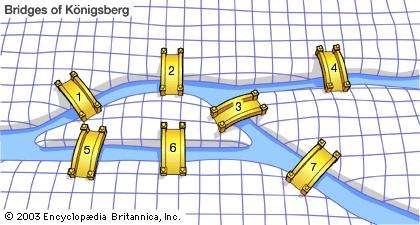
\includegraphics[width=0.9\textwidth, scale=0.9]{images/konigsberg}
	\caption[]%
	{Königsbergi hidak\\
		{\white .}\hfill\url{https://cdn.britannica.com/s:700x450/77/74877-004-6D15B0BD.jpg/}}
	\label{fig:ALAP:sm1}
\end{figure}

\subsection{Legrövidebb út probléma}

Legrövidebb út problémájára egy megoldás Dijkstra algoritmusa, mely visszatéríti a legrövidebb utat a kiinduló csúcsból az összes többi csúcsba. Negatív súlyú élek esetén nem működik. Az algoritmus komplexitása \(O(n^2)\), ahol \(n\) a csúcsok száma.



%%!TEX root = GRoutes.tex
%%%%%%%%%%%%%%%%%%%%%%%%%%%%%%%%%%%%%%%%%%%%%%%%%%%%%%%%%%%%%%%%%%%%%%%
\chapter{Gráf problémák}\label{ch:ALAP}
%%%%%%%%%%%%%%%%%%%%%%%%%%%%%%%%%%%%%%%%%%%%%%%%%%%%%%%%%%%%%%%%%%%%%%%

\begin{osszefoglal}
	Ebben a fejezetben a különböző gráfelméleti problémákat fogom röviden ismertetni.
	
\end{osszefoglal}

%%%%%%%%%%%%%%%%%%%%%%%%%%%%%%%%%%%%%%%%%%%%%%%%%%%%%%%%%%%%%%%%%%%%%%%
\section{Gráfok leszámlálása}\label{sec:ALAP:adatelem}

%%%%%%%%%%%%%%%%%%%%%%%%%%%%%%%%%%%%%%%%%%%%%%%%%%%%%%%%%%%%%%%%%%%%%%%
\section{Részgráf izomorfizmus probléma}\label{sec:ALAP:adatelem}

A részgráf izomorfizmus egy komputacionális probléma, adottak a \(H\) és \(G\) gráfok, és el kell dönteni, hogy létezik-e \(G\)-nek olyan részgráfja, amely izomorf \(H\)-val. Ennek bizonyítása egy NP-teljes feladat.

%%%%%%%%%%%%%%%%%%%%%%%%%%%%%%%%%%%%%%%%%%%%%%%%%%%%%%%%%%%%%%%%%%%%%%%
\section{Gráfok színezése}\label{sec:ALAP:adatelem}

Egy gráf színezése azt jelenti, hogy a csúcsaihoz (vagy az éleihez) színeket rendelünk (legtöbbször egy számmal reprezentáljuk), úgy, hogy két bármely két szomszédos csúcs (vagy él) különböző színű legyen.

%%%%%%%%%%%%%%%%%%%%%%%%%%%%%%%%%%%%%%%%%%%%%%%%%%%%%%%%%%%%%%%%%%%%%%%
\section{Útproblémák}\label{sec:ALAP:adatelem}

\subsection{Hamilton-kör probléma}

A Hamilton-kör egy gráfban, egy olyan kör, mely áthalad a gráf összes csúcsán. Mivel egy kör, minden csúcson egyszer fog áthaladni, kivéve az elsőt, ami egyben az utolsó is. Egy gráfot Hamilton-gráfnak nevezünk, ha tartalmaz Hamilton-kört.

Egy egyszerű gráf \(G = (X,E)\), \(n \leq 3\) csúccsal Hamilton gráf, ha \(d(x) + d(y)  \geq n\), minden nem szomszédos \(x,y \in X\) csúcsra.

Ebből kifolyólag egy gráfban a Hamilton-kör létezése elméleti szemszögből nem egy egyszerú probléma, de gyakorlati szemszögből sem, mivel NP%
\footnote{ %
	nem determinisztikusan polinomiális
}  %
-teljes. Az utazó ügynök problémája magába foglalja a Hamilton-kör létezését a gráfban.

\subsection{Minimális feszítőfa}

Egy \(fa\) egy olyan gráf, amely összefüggő és nem tartalmaz köröket. Bármely összefüggő \(G\) gráfban a feszítőfa \(G\)-nek egy olyan részgráfja, amely fa, és tartalmazza \(G\) összes csúcsát. A minimális feszítőfát meghatározhatjuk Prim algoritmusa segítségével.

Prim algoritmusa: kezdjük bármelyik csúccsal, madj válasszuk ki a hozzá tartozó legkisebb súllyal rendelkező élet. Minden iterációban kiválasztjuk az eddig vizsgált csúcsokhoz tartozó élek közül a legkisebb súllzal rendelkező élet, majd hozzáadjuk az eddig kapott fához az eddig nem vizsgált csúcspontjával együtt. Ezt addig folyatjuk, míg az összes csúcsot megvizsgáltuk.

\subsection{Kínaipostás-probléma}

Egy \(G\) gráfban, találjuk meg a legrövidebb zárt sétát, amely minden élen legalább egyszer halad át. Egy optimális megoldást találni úgy irányított, mint irányítatlan gráfban NP-teljes.

\subsection{Königsbergi hidak problémája}

Königsberg városában volt hét híd, amely összekötött két szigetet a város két partjával és egymással. A lakosok megpróbáltak úgy sétálni, hogy minden hídon egyszer és csakis egyszer haladjanak át, és érjenek vissza a kezdőpontba. Ez soha senkinek nem sikerült Euler magyarázta meg egy 1736-ban írt cikkben, hogy ez miért nem lehetséges.

Egy Euler-út egy gráfban egy olyan út, amely minden élet magába foglal, egyszer és csakis egyszer. Egy Euler-út zárt, ha ugyanabban a csúcsban végződik, mint ahonnan elindul, egyébként nyíltnak nevezzük.

Egy gráf akkor és csakis akkor tartalmaz zárt Euler-utat, ha minden csúcshoz páros számú él tartozik, valamint minden él ugyanahoz a komponenshez tartozik. Egy gráf akkor és csakis akkor tartalmaz nyílt Euler-utat, ha pontosan két csúcshoz tartozik páratlan számú él, és minden él egyazon komponenshez tartozik.

\subsection{Legrövidebb út probléma}

Dijkstra algoritmusa megoldja a legrövidebb út problémat és visszatéríti a legrövidebb utat a kiinduló csúcsból az összes többi csúcsba. Negatív súlyú élek esetén nem működik. Az algoritmus komplexitása \(O(n^2)\), ahol \(n\) a csúcsok száma.




%!TEX root = GRoutes.tex
%%%%%%%%%%%%%%%%%%%%%%%%%%%%%%%%%%%%%%%%%%%%%%%%%%%%%%%%%%%%%%%%%%%%%%%
\chapter{Az utazó ügynök problémája (TSP)}\label{ch:ALAP}
%%%%%%%%%%%%%%%%%%%%%%%%%%%%%%%%%%%%%%%%%%%%%%%%%%%%%%%%%%%%%%%%%%%%%%%


Az utazó ügynök problémája magába foglalja a Hamilton-kör létezésnek a problémáját is. Adott valamennyi város, amelyeket az utazó ügynök úgy kell meglátogasson, hogy mindegyik városba egyszer és csakis egyszer menjen be, valamint érjen vissza a kiindulási pontba, és a megtett út a legrövidebb legyen.

%%%%%%%%%%%%%%%%%%%%%%%%%%%%%%%%%%%%%%%%%%%%%%%%%%%%%%%%%%%%%%%%%%%%%%%
\section{A probléma komplexitása}\label{sec:ALAP:adatelem}

\begin{description}
	\setlength{\itemsep}{0.04mm}
	\item[P] -- azokat a problémákat foglalja magába, melyeket egy determinisztikus Turing-gép polinomiális időben képes megoldani
	\item[NP] -- azokat a problémákat foglalja magába, melyeket egy nem-determinisztikus Turing gép polinomiális időben képes megoldani. Ezeknek a megoldását polinomiális időn belül le lehet ellenőrizni determinisztikus Turing-géppel.
	\item[NP-nehéz] -- egy probléma amely "legalább olyan nehéz, mint a legnehezebb probléma az NP-ben"
	\item[NP-teljes] -- egy probléma NP-teljes ha úgy az NP, mint az NP-nehéz halmaznak is eleme, így tehát ezek a legnehezebb komputacionális problémák
\end{description}


Az utazó ügynök problémája magába foglalja a Hamilton kör problémáját is, ami NP-teljes, így tehát a TSP%
\footnote{ %
	travelling talesman problem - az utazó ügynök problémája
}  %
 is NP-teljes.

%%%%%%%%%%%%%%%%%%%%%%%%%%%%%%%%%%%%%%%%%%%%%%%%%%%%%%%%%%%%%%%%%%%%%%%
\section{Aszimmetrikus TSP}\label{sec:ALAP:adatelem}

Amennyiben irányított gráfokkal dolgozunk, abban az esetben az aszimmetrikus TSP-ről beszélünk. Nem minden TSP algoritmus működik ATSP-re is, ezért előfordulhat, hogy át kell alakítanunk a gráfot, visszavezetve a TSP-re. A visszavezetés után, \(n\) csomópontból álló ATSP egy \(2n\) csomópontból álló TSP-t fog eredményezni\cite{atsp}.

\section{Egzakt algoritmusok}\label{sec:ALAP:adatelem}

Az egzatk algoritmusok minden esetben az optimális megoldást térítik vissza, komplexitásuk azonban exponenciális. Így a csomópontok növekedésével a futási sebesség exponenciálisan fog nőni. Kutatási szemptontot leszámítva, nem lehetne ezeket az algoritmusokat átlagos felhasználói környezetben alkalmazni, ugyanis már 20 csomópont után nem lehet kivárni a megoldást. 

\subsection{Brute force}

A legegyszerűbb megközelítés, az összes permutációt kipróbálni, és kiválasztani ezek közül a legjobbat. Ennek a komplexitása azonban \(O(n!)\), így ezt már 20 városnál sem lehet alkalmazni.


\subsection{Held-Karp algoritmus}

Az algoritmus komplexitása a legrosszabb esetben \(O(n^2*2^n)\).

Legyen \(S \subseteq {2, \dots, N}\) részhalmaza a városoknak és \(d_{ij}\) az \(i\) és \(j\) városok közötti távolság. Továbbá \(c \in S\) úgy, hogy \(D(S,c)\) a minimális távolság kezdve az első várostól, meglátogatva az összes várost \(S\)-ből, majd visszaérve \(c\) városba.

Ha \(S = {c}\), akkor \(D(S,c) = d_{1,c}\), különben:

\begin{equation}
D(S,c) = min_{x \in S-c}(D(S - c,x)+d_{x,c})
\end{equation}

Ezután a minimális út az összes város érintésével:

\begin{equation}
M = min_{c \in \{2, \dots, N\}}(D(\{2, \dots, N\}, c)+d_{c, 1})
\end{equation}

Egy \{\(n_1, \dots, n_N\)\} út minimális, ha teljesíti:

\begin{equation}
M = (D(\{2, \dots, N\}, n_N)+d_{n_N, 1})
\end{equation}

\subsection{Concorde}

A \(Concorde\) TSP megoldó\cite{concorde} egzakt megoldást nyújt az útazó ügynök problémájára. ANSI C-ben íródott és a "cutting plane" módszer segítségével iteratívan oldja meg a TSP lineáris programozási relaxációit. A felhasználói grafikus felület lehetőséget ad arra, hogy különböző heurisztikus algoritmusokkal számoljuk ki a megoldást. 

A \(Concorde\) segítségével megtalálták az optimális megoldást a TSPLIB%
\footnote{ %
	a TSP-re példa adatokat tartalmazó könyvtár
}  %
mind a 110 példájára, ahol a legnagyobb 85900 várost tartalmaz.

Az alábbi eredményeket egy 2.8 GHz-es Intel Xeon processzor egy magjának használatával számolták ki, az \textit{ILOG CPLEX} lineáris programozási feladatmegoldó segítségével. Mindegyik adathalmaz 100 csomópontból áll.

\begin{table}[]
	\begin{tabular}{l|l}
		\textbf{Adathalmaz} & \textbf{Futási idő} (másodperc) \\
		\hline
		kroA100         & 0.31  \\
		kroB100         & 0.58 \\
		kroC100         & 0.30 \\   
		kroD100         & 0.33        
	\end{tabular}
\end{table}

%%%%%%%%%%%%%%%%%%%%%%%%%%%%%%%%%%%%%%%%%%%%%%%%%%%%%%%%%%%%%%%%%%%%%%%
\section{Heurisztikus algoritmusok}\label{sec:ALAP:adatelem}

\subsection{Greedy - legközelebbi szomszéd}

Mivel az egzakt algoritmusokat csak igazán kevés használati esetben lehet alkalmazni, ezért a mohó algoritmusok mellett is dönthetünk. Ezek polinomiális idő alatt elvégzik a feladatod, azonban nem mindig az optimumot térítik vissza. Az eltérés mértéke függhet azonban az implementációtól.


\begin{description}
	\setlength{\itemsep}{0.04mm}
	\item[1. lépés] -- kezdjünk egy véletlenszerűen kiválasztott csomóponttal, melyet beállítunk aktuálisnak
	\item[2. lépés] -- keressük meg a legrövidebb élet, amely összeköti az aktuális csúcsot, és egy meg nem látogatott \(V\) csúcsot
	\item[3. lépés] -- beállítjuk \(V\)-t aktuális cs]csnak
	\item[4. lépés] -- megjelöljük, hogy már meglátogattuk \(V\)-t
	\item[5. lépés] -- ha minden csomópontot meglátogattunk, akkor algoritmus vége
	\item[6. lépés] -- menjünk a 2. lépéshez
\end{description}

\subsection{2-opt algoritmus}

A 2-opt algoritmus egy lokális kereső algoritmus, mely egy meglévő utat javít fel. Ezt az algoritmust elsőként Croes javasolta 1958-ban, az alapműveletet azonban már Flood is javasolta 1956-ban. Ez abból áll, hogy egy meglévő körútból kitörlünk két élet, úgy hogy ezeknek nincs közös csúcsúk, majd a csomópontokat újra összekötjük. Erre egy lehetőség van úgy, hogy ne az előző utat kapjuk. Amennyiben az újonnan kapott körút rövidebb, megtartjuk. Ezeket a cseréket minden lehetséges kombinációra elvégezzük. Az így kapot körutat 2-optimálisnak nevezzük.

\subsection{Lin-Kernighan heurisztika}

A 2-opt algoritmus általánosítása révén született meg az egyik leghatékonyabb approximációs algoritmus a szimmetrikus TSP megoldására, a Lin-Kernighan algoritmus\cite{lin_kern}. Egy körút k-optimális, ha nem lehetséges egy rövidebb körutat kapni \(k\) darab él, más \(k\) darab éllel való helyettesítése után. Minél nagyobb a \(k\) értéke, annál valószínűbb, hogy az algoritmus végrehajtása után az optimális megoldást kapjuk, ugyanakkor nagyobb adathalmazra gyorsan növekszik a \(k\) darab élcsere ellenőrzéséhez szükséges műveletek száma. Egy hátránya tehát a \(k-opt\) algoritmusoknak, hogy futás előtt meg kell adni a \(k\) értékét. Ezt a hátrányt igyekszik kiküszöbölni a Lin-Kernighan algoritmus, azáltal, hogy futása során változtatja \(k\)-nak az értékét.

Legyen \(T\) az aktuális körút. Minden iterációban, az algoritmus igyekszik találni két \(X = \{x_1,\dots,x_k\}\) és \(Y = \{y_1,\dots,y_k\}\) élekből álló halmazt, melyekre igaz az, hogy a \(T\) körútból az \(X\)-ben található éleket az \(Y\)-ból vett élekkel helyettesítve egy jobb körutat kapunk. Ezeknek az éleknek a felcserélését \(k-opt\) lépésnek nevezzük. Ahhoz, hogy kellően hatékony algoritmust kapjunk, az \(X\) és \(Y\) halmazokhoz tartozó éleknek meg kell felelniük bizonyos kritériumoknak:

\begin{description}
	\setlength{\itemsep}{0.04mm}
	\item[(a) A szekvenciális csere kritériuma] -- \(x_i\)-nek, valamint \(y_i\)-nek rendelkezniük kell egy közös csúccsal, ugyanígy \(y_i\)-nek és \(x_{i+1}\)-nek is. Így tehát a \(x_1,y_1,x_2,y_2,\dots,x_k,y_k\) sorozat egy szomszédos élekből álló láncot alkot.
	\item[(b) A megvalósíthatósági kritérium] -- szükséges továbbá, hogy \(x_i = (t_{\{2i-1\}},t_{\{2i\}})\) úgy legyen kiválasztva, hogy ha a \(t_{\{2i\}}\)-t csatlakoztatjuk a \(t_1\)-hez, az így kapott gráf körút maradjon. Ez a kritérium az algoritmus futási idejének csökkentéséért, valamint a kódolás leegyszerűsítéséért lett bevonva.
	\item[(c) A pozitív nyereség kritériuma] -- az \(y_i\)-t úgy kell kiválasztani, hogy a nyereség a javaslot cserék után pozitív maradjon. Ez a feltétel kulcsfontosságú az algoritmus hatékonyságának szempontjából.
	\item[(d) A diszjunktivitás kritérium] -- az \(X\) és \(Y\) halmazoknak diszjunktnak kell lenniük
\end{description}

%%!TEX root = GRoutes.tex
%%%%%%%%%%%%%%%%%%%%%%%%%%%%%%%%%%%%%%%%%%%%%%%%%%%%%%%%%%%%%%%%%%%%%%%
\chapter{TSP algoritmusok}\label{ch:ALAP}
%%%%%%%%%%%%%%%%%%%%%%%%%%%%%%%%%%%%%%%%%%%%%%%%%%%%%%%%%%%%%%%%%%%%%%%

\begin{osszefoglal}
	Ebben a fejezetben az utazó ügynök problémáját megoldó algoritmusokat fogom részletesen tárgyalni.
	
\end{osszefoglal}

%%%%%%%%%%%%%%%%%%%%%%%%%%%%%%%%%%%%%%%%%%%%%%%%%%%%%%%%%%%%%%%%%%%%%%%
\section{Egzakt algoritmusok}\label{sec:ALAP:adatelem}

\subsection{Brute force}

A legegyszerűbb megközelítés, az összes permutációt kipróbálni, és kiválasztani ezek közül a legjobbat. Ennek a komplexitása azonban \(O(n!)\), így ezt már 20 városnál se lehet alkalmazni.


\subsection{Held-Karp algoritmus}

Az algoritmus komplexitása a legrosszabb esetben \(O(n^2*2^n)\).

Legyen \(S \subseteq {2, \dots, N}\) részhalmaza a városoknak, és \(c \in S\) úgy, hogy \(D(S,c)\) a minimális távolság kezdve az első várostól, meglátogatva az összes várost \(S\)-ből, majd visszaérve \(c\) városba.

ha \(S = {c}\), akkor \(D(S,c) = d_{1,c}\), különben:

\begin{equation}
D(S,c) = min_{x \in S-c}(D(S - c,x)+d_{x,c})
\end{equation}

Ezután a minimális út az összes város érintésével:

\begin{equation}
M = min_{c \in \{2, \dots, N\}}(D(\{2, \dots, N\}, c)+d_{c, 1})
\end{equation}

Egy \{\(n_1, \dots, n_N\)\} út minimális, ha teljesíti:

\begin{equation}
M = (D(\{2, \dots, N\}, n_N)+d_{n_N, 1})
\end{equation}

\subsection{Concorde algoritmus}

A \(Concorde\) algoritmus egzakt megoldást nyújt a TSP-re. Ennek segítségével megtalálták az optimális megoldást a TSPLIB%
\footnote{ %
	a TSP-re példa adatokat tartalmazó könyvtár
}  %
 mind a 110 példájára, ahol a legnagyobb 85900 várost tartalmaz.

%%%%%%%%%%%%%%%%%%%%%%%%%%%%%%%%%%%%%%%%%%%%%%%%%%%%%%%%%%%%%%%%%%%%%%%
\section{Heurisztikus algoritmusok}\label{sec:ALAP:adatelem}

\subsection{Greedy - legközelebbi szomszéd}

\begin{description}
	\setlength{\itemsep}{0.04mm}
	\item[1. lépés] -- kezdjünk egy véletlenszerűen kiválasztott csomóponttal, melyet beállítunk aktuálisnak
	\item[2. lépés] -- keressük meg a legrövidebb élet, amely összeköti az aktuális csúcsot, és egy meg nem látogatott \(V\) csúcsot
	\item[3. lépés] -- beállítjuk \(V\)-t aktuális cs]csnak
	\item[4. lépés] -- megjelöljük, hogy már meglátogattuk \(V\)-t
	\item[5. lépés] -- ha minden csomópontot meglátogattunk, akkor algoritmus vége
	\item[6. lépés] -- menjünk a 2. lépéshez
\end{description}

\subsection{Lin-Kernighan heurisztika}

%!TEX root = GRoutes.tex
%%%%%%%%%%%%%%%%%%%%%%%%%%%%%%%%%%%%%%%%%%%%%%%%%%%%%%%%%%%%%%%%%%%%%%%
\chapter{Technológiák}
%%%%%%%%%%%%%%%%%%%%%%%%%%%%%%%%%%%%%%%%%%%%%%%%%%%%%%%%%%%%%%%%%%%%%%%

\begin{osszefoglal}
	Ebben a fejezetben, a projekt elkészítése során felhasznált technológiákat ismertetem.
	
\end{osszefoglal}

%%%%%%%%%%%%%%%%%%%%%%%%%%%%%%%%%%%%%%%%%%%%%%%%%%%%%%%%%%%%%%%%%%%%%%%
\section{Android}

\begin{figure}
	\centering
	\setlength{\abovecaptionskip}{0pt}
	\setlength{\belowcaptionskip}{0pt}
	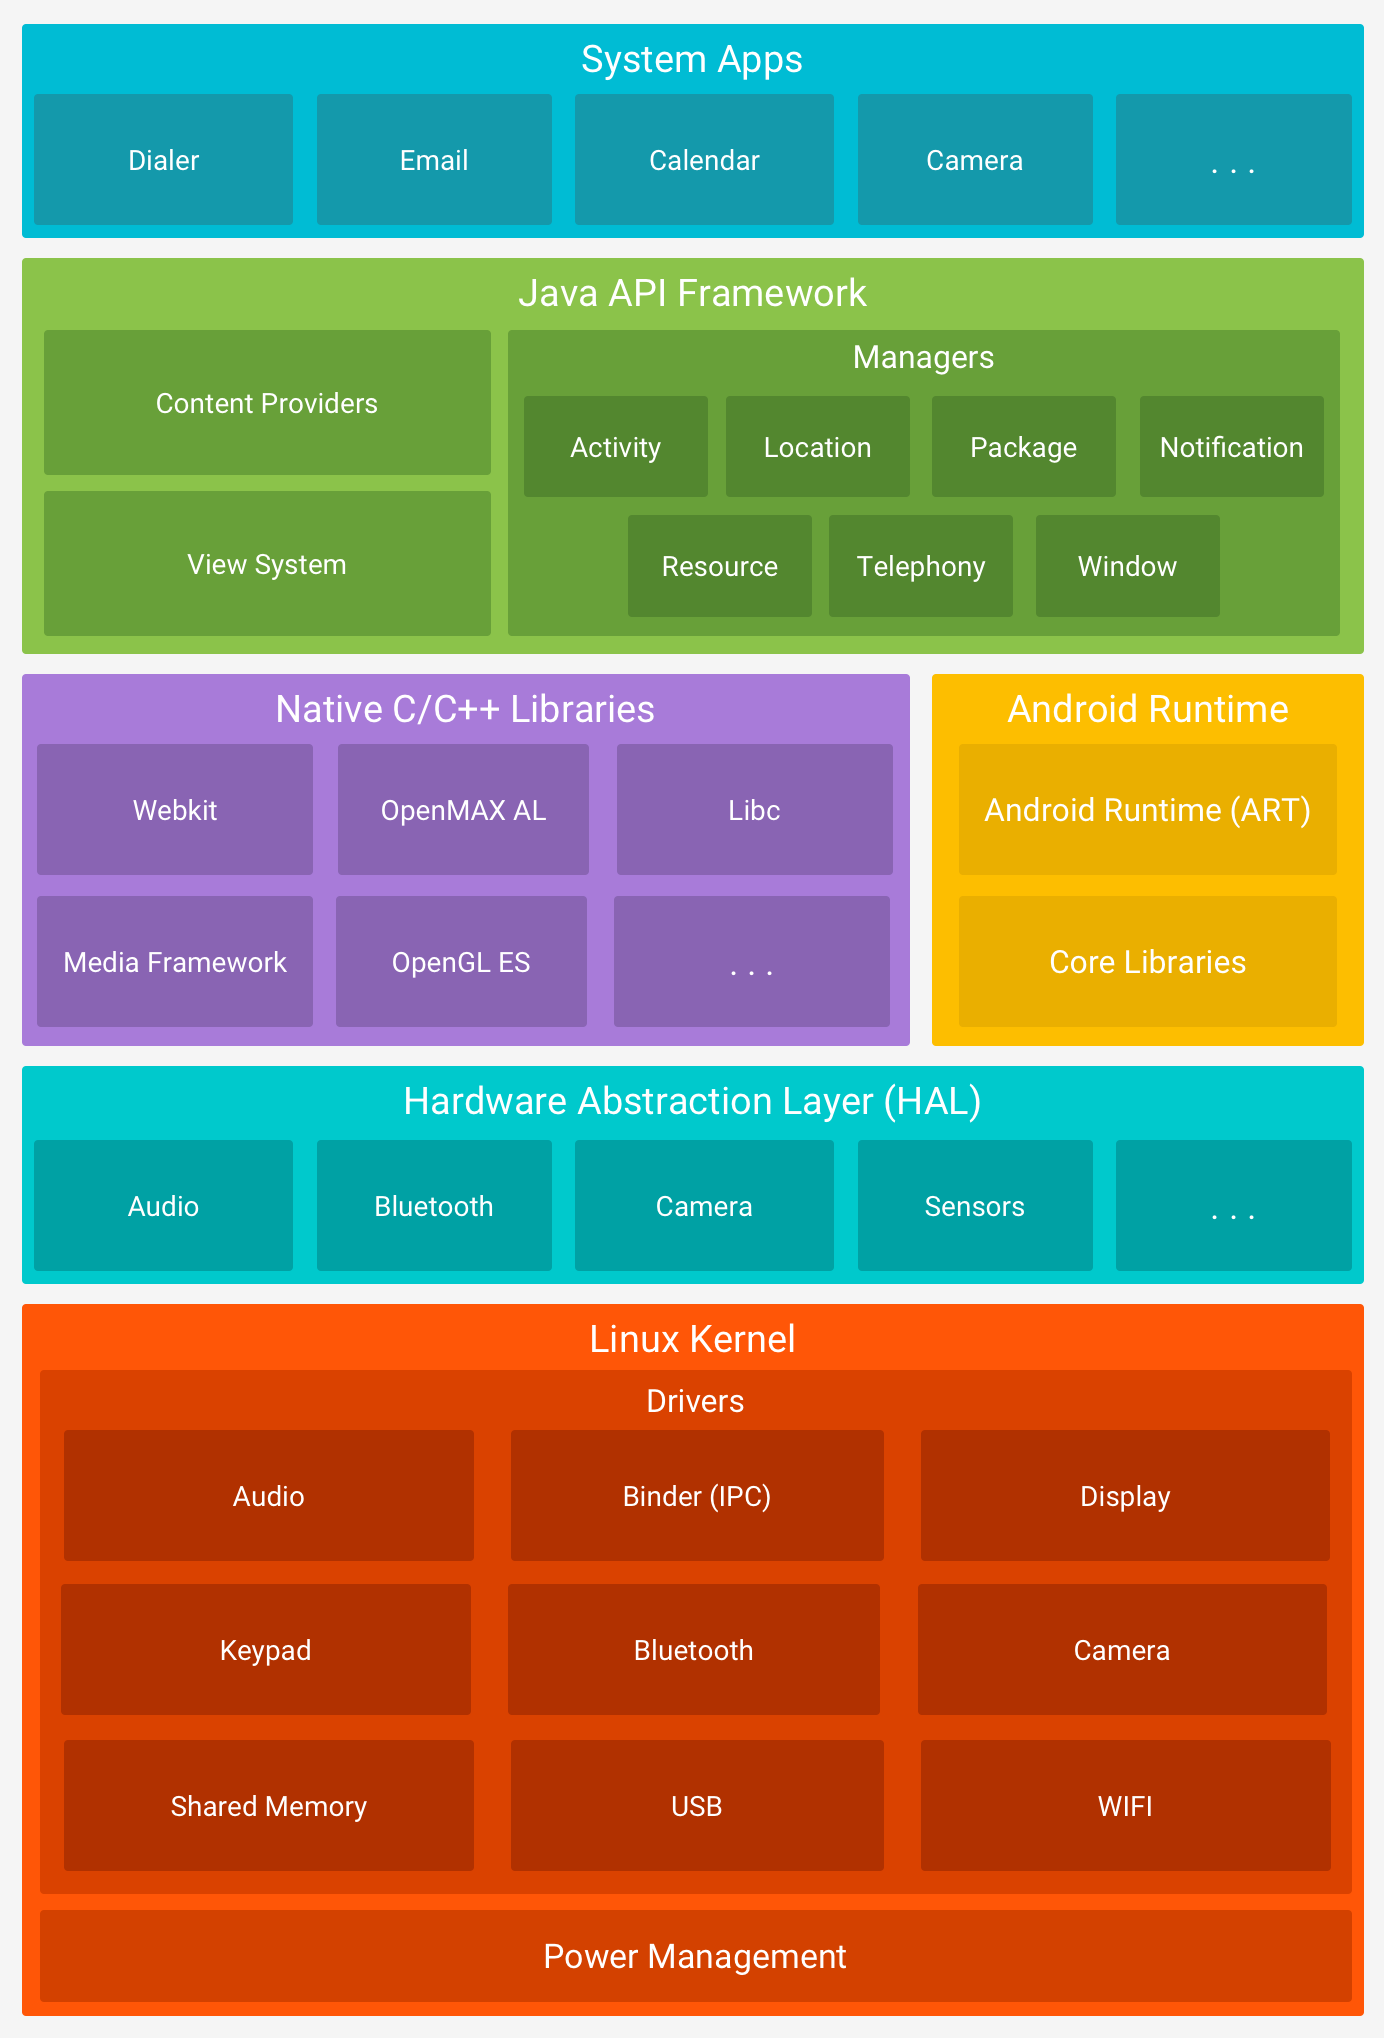
\includegraphics[width=0.9\textwidth, scale=0.9]{images/android}
	\caption{Android\label{fig:ALAP:sm2}}
\end{figure}

Az Android egy nyílt forráskódú, Linux kernel alapú többfelhasználós operációs rendszer, ahol minden applikáció egy külön felhasználó. Hivatalos nyelvei a Java és a Kotlin. Alapértelmezetten, a rendszer minden applikációnak kioszt egy egyedi Linux felhasználói ID-t (az ID-t csak a rendszer használja, és ismeretlen az applikáció számára). Az operációs rendszer úgy osztja ki a hozzáfárési jogokat az applikáció állományai számára, hogy csak az a felhasználói ID férjen hozzájuk, amivel az adott applikáció rendelkezik. Minden folyamat (process) rendelkezik a saját virtuális gépével, tehát minden applikáció kódja egymástól teljesen izoláltan fut. Alapértelmezetten minden applikáció a saját Linux folyamatában fut. Az Android operációs rendszer elindítja a folyamatot, amikor az applikáció valamelyik komponensének szüksége van rá, majd leállítja azt, mikor többé már nincs rá szükség, vagy ha a rendszernek mermóriát kell lefoglalnia, más applikációk számára. Az Android operációs rendszer “a legkevesebb kiváltság elvét” (“the principle of least privilige”) alkalmazza, tehát alapértelmezetten, minden applikációnak csak azokhoz a komponensekhez van hozzáférése, amik szükségesek a feladatának elvégzéséhez, és semmi egyébhez.

Egy android applikációnak négy fajta komponense lehet: Activity, Service, Broadcast receiver, Content provider. Ezek közül az Activity szolgál a felhasználóval történő interakció eszközéül, ez ugyanis egy felhasználói felülettel rendelkező képernyő. Activity-k, Service-k és Broadcast receiver-ek egy aszinkron üzenet által aktiválódnak, amit Intent-nek (szándék) nevezünk.

Az Activity egy osztály (class), amely a logikát tartalmazza, a felhasználói felületért azonban egy ehhez tartozó XML állomány felel, ami a különböző UI elemeket (gombok, szövegdobozok, konténerek) tartalmazza.

Az AndroidManifest.xml egy konfigurációs állomány, ami a projekt gyökér könyvtárában található. Itt vannak deklarálva az applikáció komponensei, valamint a szükséges hozzáférési jogokat is itt kell feltünteni.



The Linux Kernel
The foundation of the Android platform is the Linux kernel. For example, the Android Runtime (ART) relies on the Linux kernel for underlying functionalities such as threading and low-level memory management.

Using a Linux kernel allows Android to take advantage of key security features and allows device manufacturers to develop hardware drivers for a well-known kernel.

Hardware Abstraction Layer (HAL)
The hardware abstraction layer (HAL) provides standard interfaces that expose device hardware capabilities to the higher-level Java API framework. The HAL consists of multiple library modules, each of which implements an interface for a specific type of hardware component, such as the camera or bluetooth module. When a framework API makes a call to access device hardware, the Android system loads the library module for that hardware component.

Android Runtime
For devices running Android version 5.0 (API level 21) or higher, each app runs in its own process and with its own instance of the Android Runtime (ART). ART is written to run multiple virtual machines on low-memory devices by executing DEX files, a bytecode format designed specially for Android that's optimized for minimal memory footprint. Build toolchains, such as Jack, compile Java sources into DEX bytecode, which can run on the Android platform.

Some of the major features of ART include the following:

Ahead-of-time (AOT) and just-in-time (JIT) compilation
Optimized garbage collection (GC)
On Android 9 (API level 28) and higher, conversion of an app package's Dalvik Executable format (DEX) files to more compact machine code.
Better debugging support, including a dedicated sampling profiler, detailed diagnostic exceptions and crash reporting, and the ability to set watchpoints to monitor specific fields
Prior to Android version 5.0 (API level 21), Dalvik was the Android runtime. If your app runs well on ART, then it should work on Dalvik as well, but the reverse may not be true.

Android also includes a set of core runtime libraries that provide most of the functionality of the Java programming language, including some Java 8 language features, that the Java API framework uses.

Native C/C++ Libraries
Many core Android system components and services, such as ART and HAL, are built from native code that require native libraries written in C and C++. The Android platform provides Java framework APIs to expose the functionality of some of these native libraries to apps. For example, you can access OpenGL ES through the Android framework’s Java OpenGL API to add support for drawing and manipulating 2D and 3D graphics in your app.

If you are developing an app that requires C or C++ code, you can use the Android NDK to access some of these native platform libraries directly from your native code.

Java API Framework
The entire feature-set of the Android OS is available to you through APIs written in the Java language. These APIs form the building blocks you need to create Android apps by simplifying the reuse of core, modular system components and services, which include the following:

A rich and extensible View System you can use to build an app’s UI, including lists, grids, text boxes, buttons, and even an embeddable web browser
A Resource Manager, providing access to non-code resources such as localized strings, graphics, and layout files
A Notification Manager that enables all apps to display custom alerts in the status bar
An Activity Manager that manages the lifecycle of apps and provides a common navigation back stack
Content Providers that enable apps to access data from other apps, such as the Contacts app, or to share their own data
Developers have full access to the same framework APIs that Android system apps use.

System Apps
Android comes with a set of core apps for email, SMS messaging, calendars, internet browsing, contacts, and more. Apps included with the platform have no special status among the apps the user chooses to install. So a third-party app can become the user's default web browser, SMS messenger, or even the default keyboard (some exceptions apply, such as the system's Settings app).

The system apps function both as apps for users and to provide key capabilities that developers can access from their own app. For example, if your app would like to deliver an SMS message, you don't need to build that functionality yourself—you can instead invoke whichever SMS app is already installed to deliver a message to the recipient you specify.

%%%%%%%%%%%%%%%%%%%%%%%%%%%%%%%%%%%%%%%%%%%%%%%%%%%%%%%%%%%%%%%%%%%%%%%
\section{Gradle}\label{sec:ALAP:adatelem}

A Gradle egy nyílt forráskódú projektépítő eszköz (build automation tool). A Groovy, vagy Kotlin nyelvű scriptekbe, megadhatjuk a projektünk külső függöségeit (például API-k, library-k), melyeket letölti, majd lekompillálja és lefordítja a forráskódot.

\subsection{Teljesítmény}

\begin{description}
	\setlength{\itemsep}{0.04mm}
	\item[Inkrementális build] -- a Gradle leellenőrzi a build-ek futtatása között, hogy változtak-e a bemeneti adatok, a kimeneti adatok, vagy egy feladat implementációja az utolsó build meghívása óta. Ha nem változtak, akkor a feladatot (task) nem hajtja végre még egyszer. Egy faladat konfigurációja is bemeneti adatként tekintendő.
	\item[Inktrementális részfeladatok] -- részfeladatok esetén is számon tartja, hogy változtak-e a bemeneti, valamint a kimeneti adatok, így pontosan meg tudja állaptíani, hogy mi változott, így nem biztos, hogy mindent újra kell build-elnie.
	\item[Párhuzamos végrehajtás] -- lehetőség van a feladatok és a részfeladatok párhuzamos végrehajtására, ami jelentősen növeli a build végrehajtásának sebességét.
	\item[Függőségek párhuzamos letöltése] -- a függőségek letőltése párhuzamosan zajlik, igény szerint, vagyis csak akkor, amikor szükség van ezekre.
\end{description}

\subsection{Függőségkezelés}

\begin{description}
	\setlength{\itemsep}{0.04mm}
	\item[Tranzitív függőségek] -- függőség menedzselő rendszer lévén, a Gradle gondoskodik a tranzitív függőségek letöltéséről, valamint kezeléséről.
	\item[Külső függőségek] -- amikor a függőségek "távoli raktárakban" (remote repository) találhatóak, akkor ezeket eltárolja egy lokálisan, így egymást követő build-ek során újra felhasználja, elkerülvén a felesleges hálózati forgalmat.
\end{description}

\subsection{Android alkalmazások}

Az Andoid Studio-hoz (az android hivatalos fejlesztői környezete) tartozó Gradle kiegészítő az android alkalmazások hivatalos build eszköze, melyet az android fejlesztői csapata tart karban.

\begin{description}
	\setlength{\itemsep}{0.04mm}
	\item[Teljes integráció az Android Studio-val] -- a Gradle olyannyira mélyen van integrálva az Android Studio-ba, hogy az utóbbinak nincs is saját build eszköze, hanem őt bízza meg a build-elési feladatokkal.
	\item[Automatikus aláírás] -- automatikusan aláírja a fejlesztett applikációkat, ami szükséges ahhoz, hogy feltöltsük ezeket a Google Play áruházba.
	\item[Multidex támogatás] -- ez lehetővé teszi, hogy meghaladjuk a 65000-es metódusszám limitet, mely az Anroid DEX állományokra vonatkozik és az applikáció .apk-ba való csomagolásakor történik az ellenőrzése.
\end{description}

%%%%%%%%%%%%%%%%%%%%%%%%%%%%%%%%%%%%%%%%%%%%%%%%%%%%%%%%%%%%%%%%%%%%%%%
\section{Firebase}\label{sec:ALAP:szerkeszt}

A felhasználók adatainak, beállításainak tárolására, kezelésére a Firestore nevű no-sql (.json) alapú adatbázist használtam, mely a CRUD%
\footnote{ %
	create, read, update, delete
}  %
 műveletekhez is biztosít metódusokat. Logikai éptőelemei a kollekciók (collection) és a dokumentumok (document). Az előbbi tartalmazhat dokumentumokat, míg az utóbbi alkollekciókat, vagy magukat az adatokat. Az adatok kulcs, érték párok, az értékek lehetnek számok, karakterláncok, tömbök, geopontok vagy akár sajátos osztályok. Amennyiben sajátos osztály akarunk használni, annak rendelkeznie kell egy publikus konstruktorral, melynek nincsenek paraméterei, valamint az attribútumokhoz kell tartozzon egy-egy publikus „getter”%
 \footnote{ %
 	egy paraméter nélküli metódus, mely egy attribútumot térít vissza - példa: String getName()
 }  %
 metódus. Az adatbázisban található adatokhoz való hozzáférést egy szabállyal kell megadni, amelyet a szerver leellenőriz a CRUD műveletek végrehajtása esetén.

A felhasználók menedzselésére, mint a regisztráció, bejelentkezés, e-mail cím aktiválása, elfelejtett jelszó visszaállítása, a Firebase Authentication szolgáltatást használtam.



Users in Firebase Projects
A Firebase User object represents the account of a user who has signed up to an app in your Firebase project. Apps usually have many registered users, and every app in a Firebase project shares a user database.

A Firebase User instance is independent from a Firebase Auth instance. This means that you can have several references to different users within the same context and still call any of their methods.

User properties
A Firebase User has a fixed set of basic properties—a unique ID, a primary email address, a name and a photo URL—stored in the project's user database, that can be updated by the user (iOS, Android, web). You cannot add other properties to the Firebase User object directly; instead, you can store the additional properties in your Firebase Realtime Database.

The first time a user signs up to your app, the user's profile data is populated using the available information:

If the user signed up with an email address and password, only the primary email address property is populated
If the user signed up with a federated identity provider, such as Google or Facebook, the account information made available by the provider is used to populate the Firebase User's profile
If the user signed up with your custom auth system, you must explicitly add the information you want to the Firebase User's profile
Once a user account has been created, you can reload the user's information to incorporate any changes the user might have made on another device.

Sign-in providers
You can sign in users to your Firebase apps using several methods: email address and password, federated identity providers, and your custom auth system. You can associate more than one sign-in method with a user: for example, a user can sign in to the same account using an email address and a password, or using Google Sign-In.

A Firebase User instance keeps track of every provider linked to the user. This allows you to update empty profile's properties using the information given by a provider. See Managing Users (iOS, Android, web).

The current user
When a user signs up or signs in, that user becomes the current user of the Auth instance. The Firebase Auth instance persists the user's state, so that refreshing the page (in a browser) or restarting the application doesn't lose the user's information.

When the user signs out, the Auth instance stops keeping a reference to the User object and no longer persists its state; there is no current user. However, the user instance continues to be completely functional: if you keep a reference to it, you can still access and update the user's data.

The user lifecycle
The recommended way to track the current state of the Firebase Auth instance is by using listeners (also called "observers" in JavaScript). An Auth listener gets notified any time something relevant happens to the Auth object. See Managing Users (iOS, Android, web).

An Auth listener gets notified in the following situations:

The Auth object finishes initializing and a user was already signed in from a previous session, or has been redirected from an identity provider's sign-in flow
A user signs in (the current user is set)
A user signs out (the current user becomes null)
The current user's access token is refreshed. This case can happen in the following conditions:
The access token expires: this is a common situation. The refresh token is used to get a new valid set of tokens.
The user changes their password: Firebase issues new access and refresh tokens and renders the old tokens expired. This automatically expires the user's token and/or signs out the user on every device, for security reasons
The user re-authenticates: some actions require that the user's credentials are recently issued; such actions include deleting an account, setting a primary email address, and changing a password. Instead of signing out the user and then signing in the user again, get new credentials from the user, and pass the new credentials to the reauthenticate method of the User object.
Auth tokens
When you perform authentication with Firebase, there are three kinds of auth tokens you might encounter:

Firebase ID tokens	Created by Firebase when a user signs in to a Firebase app. These tokens are signed JWTs that securely identify a user in a Firebase project. These tokens contain basic profile information for a user, including the user's ID string, which is unique to the Firebase project. Because the integrity of ID tokens can be verified, you can send them to a backend server to identify the currently signed-in user.
Identity provider tokens	Created by federated identity providers, such as Google and Facebook. These tokens can have different formats, but are often OAuth 2.0 access tokens. Firebase apps use these tokens to verify that users have successfully authenticated with the identity provider, and then convert them into credentials usable by Firebase services.
Firebase custom tokens	Created by your custom auth system to allow users to sign in to a Firebase app using your auth system. Custom tokens are JWTs signed using a service account's private key. Firebase apps use these tokens much like they use the tokens returned from federated identity providers.



Cloud Firestore is a flexible, scalable database for mobile, web, and server development from Firebase and Google Cloud Platform. Like Firebase Realtime Database, it keeps your data in sync across client apps through realtime listeners and offers offline support for mobile and web so you can build responsive apps that work regardless of network latency or Internet connectivity. Cloud Firestore also offers seamless integration with other Firebase and Google Cloud Platform products, including Cloud Functions.

Cloud Firestore is currently in beta release. Feature availability and support for product integrations and platforms will continue to improve as the product matures. For more information on existing limitations in Cloud Firestore, see the limits and quotas documentation
GET STARTED

Key capabilities
Flexibility	The Cloud Firestore data model supports flexible, hierarchical data structures. Store your data in documents, organized into collections. Documents can contain complex nested objects in addition to subcollections.
Expressive querying	In Cloud Firestore, you can use queries to retrieve individual, specific documents or to retrieve all the documents in a collection that match your query parameters. Your queries can include multiple, chained filters and combine filtering and sorting. They're also indexed by default, so query performance is proportional to the size of your result set, not your data set.
Realtime updates	Like Realtime Database, Cloud Firestore uses data synchronization to update data on any connected device. However, it's also designed to make simple, one-time fetch queries efficiently.
Offline support	Cloud Firestore caches data that your app is actively using, so the app can write, read, listen to, and query data even if the device is offline. When the device comes back online, Cloud Firestore synchronizes any local changes back to Cloud Firestore.
Designed to scale	Cloud Firestore brings you the best of Google Cloud Platform's powerful infrastructure: automatic multi-region data replication, strong consistency guarantees, atomic batch operations, and real transaction support. We've designed Cloud Firestore to handle the toughest database workloads from the world's biggest apps.
How does it work?


Cloud Firestore is a cloud-hosted, NoSQL database that your iOS, Android, and web apps can access directly via native SDKs. Cloud Firestore is also available in native Node.js, Java, Python, and Go SDKs, in addition to REST and RPC APIs.

Following Cloud Firestore's NoSQL data model, you store data in documents that contain fields mapping to values. These documents are stored in collections, which are containers for your documents that you can use to organize your data and build queries. Documents support many different data types, from simple strings and numbers, to complex, nested objects. You can also create subcollections within documents and build hierarchical data structures that scale as your database grows. The Cloud Firestore data model supports whatever data structure works best for your app.

Additionally, querying in Cloud Firestore is expressive, efficient, and flexible. Create shallow queries to retrieve data at the document level without needing to retrieve the entire collection, or any nested subcollections. Add sorting, filtering, and limits to your queries or cursors to paginate your results. To keep data in your apps current, without retrieving your entire database each time an update happens, add realtime listeners. Adding realtime listeners to your app notifies you with a data snapshot whenever the data your client apps are listening to changes, retrieving only the new changes.

Protect access to your data in Cloud Firestore with Firebase Authentication and Cloud Firestore Security Rules for Android, iOS, and JavaScript, or Identity and Access Management (IAM) for server-side languages.

Implementation path
Integrate the Cloud Firestore SDKs	Quickly include clients via Gradle, CocoaPods, or a script include.
Secure your data	Use Cloud Firestore Security Rules or Identity and Access Management (IAM) to secure your data for mobile/web and server development, respectively.
Add Data	Create documents and collections in your database.
Get Data	Create queries or use realtime listeners to retrieve data from the database.

%%%%%%%%%%%%%%%%%%%%%%%%%%%%%%%%%%%%%%%%%%%%%%%%%%%%%%%%%%%%%%%%%%%%%%%
\section{Térkép}\label{sec:ALAP:szerkeszt}

\subsection{Distance Matrix API}

ntroduction
The Distance Matrix API is a service that provides travel distance and time for a matrix of origins and destinations. The API returns information based on the recommended route between start and end points, as calculated by the Google Maps API, and consists of rows containing duration and distance values for each pair.

Note: This service does not return detailed route information. Route information can be obtained by passing the desired single origin and destination to the Directions API.

Before you begin
This document is intended for developers who wish to compute travel distance and time between a number of points within maps provided by one of the Google Maps APIs. It provides an introduction to using the API and reference material on the available parameters.

Before you start developing with the Distance Matrix API, review the authentication requirements (you need an API key) and the API usage and billing information (you need to enable billing on your project).

Distance Matrix Requests
A Distance Matrix API request takes the following form:

https://maps.googleapis.com/maps/api/distancematrix/outputFormat?parameters
where outputFormat may be either of the following values:

json (recommended), indicates output in JavaScript Object Notation (JSON); or
xml, indicates output as XML.
Note: URLs must be properly encoded to be valid and are limited to 8192 characters for all web services. Be aware of this limit when constructing your URLs. Note that different browsers, proxies, and servers may have different URL character limits as well.

HTTPS or HTTP
Security is important and HTTPS is recommended whenever possible, especially for applications that include sensitive user data, such as a user's location, in requests. Using HTTPS encryption makes your application more secure, and more resistant to snooping or tampering.

If HTTPS is not possible, to access the Distance Matrix API over HTTP, use:

http://maps.googleapis.com/maps/api/distancematrix/outputFormat?parameters
Request Parameters
Certain parameters are required while others are optional. As is standard in URLs, all parameters are separated using the ampersand  character.

Request Parameters
Certain parameters are required while others are optional. As is standard in URLs, all parameters are separated using the ampersand character.

Required parameters
origins — The starting point for calculating travel distance and time. You can supply one or more locations separated by the pipe character (|), in the form of an address, latitude/longitude coordinates, or a place ID:
If you pass an address, the service geocodes the string and converts it to a latitude/longitude coordinate to calculate distance. This coordinate may be different from that returned by the Geocoding API, for example a building entrance rather than its center.
origins=Bobcaygeon+ON|24+Sussex+Drive+Ottawa+ON
If you pass latitude/longitude coordinates, they are used unchanged to calculate distance. Ensure that no space exists between the latitude and longitude values.
origins=41.43206,-81.38992|-33.86748,151.20699
If you supply a place ID, you must prefix it with placeid. You can only specify a place ID if the request includes an API key or a Google Maps APIs Premium Plan client ID. You can retrieve place IDs from the Geocoding API and the Places SDK (including Place Autocomplete). For an example using place IDs from Place Autocomplete, see Place Autocomplete and Directions. For more about place IDs, see the place ID overview.
origins=placeid:ChIJ3S-JXmauEmsRUcIaWtf4MzE
Alternatively, you can supply an encoded set of coordinates using the Encoded Polyline Algorithm. This is particularly useful if you have a large number of origin points, because the URL is significantly shorter when using an encoded polyline.
Encoded polylines must be prefixed with enc and followed by a colon. For example: origins=enc:gfoEtohhU:
You can also include multiple encoded polylines, separated by the pipe character . For example: origins=
destinations — One or more locations to use as the finishing point for calculating travel distance and time. The options for the destinations parameter are the same as for the origins parameter, described above.
key — Your application's API key. This key identifies your application for purposes of quota management. Learn how to get a key.
Note: Google Maps APIs Premium Plan customers may use either an API key, or a valid client ID and digital signature, in your Distance Matrix requests. Get more information on authentication parameters for Premium Plan customers

\subsection{Directions API}

A csomópontok közti távolságok mátrixának lekérdezésére a Distance Matrix API-t, valamint két csomópont közötti útvonal meghatározására a Directions API-t használtam.

The Distance Matrix API is a service that provides travel distance and time for a matrix of origins and destinations. The API returns information based on the recommended route between start and end points, as calculated by the Google Maps API, and consists of rows containing duration and distance values for each pair.


The Directions API is a service that calculates directions between locations using an HTTP request.

This video illustrates the use of the Directions API to help people find their way. The video includes advice on proxying the web service via your server when you're using the API in a mobile app, to protect your API key.


With the Directions API, you can:

Search for directions for several modes of transportation, including transit, driving, walking or cycling.
Return multi-part directions using a series of waypoints.
Specify origins, destinations, and waypoints as text strings (e.g. "Chicago, IL" or "Darwin, NT, Australia"), or as latitude/longitude coordinates, or as place IDs.
The API returns the most efficient routes when calculating directions. Travel time is the primary factor optimized, but the API may also take into account other factors such as distance, number of turns and many more when deciding which route is the most efficient.

Tip: Calculating directions is a time and resource intensive task. Whenever possible, use the service described here to calculate known addresses ahead of time and store the results in a temporary cache of your own design.

Note: This service is not designed to respond in real time to user input. For dynamic directions calculations (for example, within a user interface element), consult the documentation for the Maps JavaScript API Directions Service.


%!TEX root = GRoutes.tex
%%%%%%%%%%%%%%%%%%%%%%%%%%%%%%%%%%%%%%%%%%%%%%%%%%%%%%%%%%%%%%%%%%%%%%%
\chapter{GRoutes - alkalmazás bemutatása}\label{ch:ALAP}
%%%%%%%%%%%%%%%%%%%%%%%%%%%%%%%%%%%%%%%%%%%%%%%%%%%%%%%%%%%%%%%%%%%%%%%

\begin{osszefoglal}
	Ebben a fejezetben a GRoutes android applikációt fogom bemutatni úgy technikai, mint funkcionális szempontból.
	
\end{osszefoglal}

%%%%%%%%%%%%%%%%%%%%%%%%%%%%%%%%%%%%%%%%%%%%%%%%%%%%%%%%%%%%%%%%%%%%%%%
\section{Funkcionalitások}\label{sec:ALAP:adatelem}

\subsection{Bejelentkezés}

\begin{wrapfigure}{l}{0.4\linewidth}
	\centering
	\setlength{\abovecaptionskip}{0pt}
	\setlength{\belowcaptionskip}{0pt}
	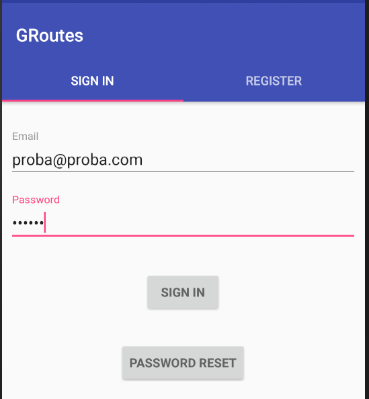
\includegraphics[width=0.4\textwidth]{images/login}
	\caption{Bejelentkezési felület\label{fig:ALAP:sm2}}
\end{wrapfigure}

Az alkalmazás elindítása után egy bejelentkezési felület fogadja a felhasználót. Itt kell megadni az e-mail címet, valamint a jelszót amivel a felhasználó regisztrált. Amennyiben elfelejtette a jelszavát, az "elfelejtett jelszó" gomb megnyomásával lehetőség van egy jelszó-visszaállító e-mail kiküldésére. 

Ha egy új felhasználó szeretné igénybe venni az applikáció szolgáltatásait, akkor regisztrálnia kell. Ezt megteheti a regisztráció lapra való navigálás után, melyet a cím megérintésével, vagy a képernyőn az ujjának balra történő húzásával érheti el. Az e-mail cím és az új jelszó megadása után, a felhasználó egyből a főmenübe érkezik, mindeközben azonban egy aktivációs e-mailt is kap arra a címére, amivel regisztrált. A későbbiekben csak akkor fog tudni bejelentkezni, ha a kapott emailben az URL%
\footnote{ %
	Uniform Resource Locator, más néven webcím
}  %
-re klikkelve aktiválja a felhasználóját.

\subsection{Főmenü}

A főmenüből négy különböző oldalra navigálhatunk tovább: a keresési felület, a régebbi keresések megtekintése, a kedvencek menedzselése, valamint a beállítások. Az ötödik (csoportok) oldal egy jövőbeli funkcionalitás kifejlesztésére van fenntartva.

\subsection{Keresési felület}

Ezen a felületen van lehetőségünk útvonalak, helyszínek keresésére. A "+" gomb megjelenít egy új mezőt, ahol további címeket adhatunk meg. A "nagyító" gomb a térkép felületre navigál, és kirajzolja a tervezett útvonalat. A keresés elindítása előtt, minden cím mellett van egy "térkép" gomb, ennek segítségével tudjuk megnézni, hogy valóban az az a hely, amire gondoltunk.

\subsection{Kedvencek}
 
 Itt jelennek meg az általunk manuálisan elmentett utak, helyszínek. Minden bejegyzésnél négy gomb jelenik meg, ezeknek az funkcióik a következők:
 
 \begin{description}
 	\setlength{\itemsep}{0.04mm}
 	\item[térkép] -- megjeleníti a térkép felületet, ahol ráközelít a helyszín koordinátáira, vagy kirajzolja az útvonalat.
 	\item[nagyító] -- a keresési felülethez navigál és kitölti a keresési mezőket, az útvonal csomópontjaíval, így a felhasználó könnyedén módosíthatja útvonaltervét.
 	\item[ceruza] -- módosítja a bejegyzés nevét.
 	\item[szemetes veder] -- törli a bejegyzést, ezáltal az adatbázisból is törlődni fog.
 \end{description}

\subsection{Múltbeli keresések}

A keresési felület eredményéül kapott útvonalak megjelennek a múltbeli keresések menüpont alatt, nevüket a keresési dátum és időpont alkotja. A bejegyzéseknél a "Kedvenceknél" tárgyalt gombok találhatóak, azonos funkcióval, azzal a kivétellel, hogy a "ceruza" gombot a "csillag" helyettesíti, melynek segítségével elmenthetünk egy útvonalat a kedvencek közé.

\subsection{Beállítások}

Itt ki tudjuk választani a limitet, hogy mennyi csomópont esetén, melyik algoritmust használja az alkalmazás. A megadott számnál kisebb vagy egyenlő számú csomópontok esetén a \(Concorde\) nevű egzakt megoldásokat nyújtó algoritmus fogja kiszámolni az ideális útvonalat. Ez az algoritmus a legpontosabb megoldásokat nyújtja, azonban az "utazó ügynök" problémájának komplexitása miatt, a csomópontok növekedésével, a végrehajtási idő is exponenciálisan növekszik. Amennyiben a felhasználó nagyon sok csomóponttal szeretne dolgozni, és fontosabb neki az, hogy belátható időn belül egy elfogadható megoldást kapjon, de nem probléma, ha nem a leghatékonyabb útvonal rajzolódik ki, akkor a megadott szám feletti mennyiségű csomópontok esetén, az applikáció egy úgynevezett \(greedy\)%
\footnote{ %
	mohó
}  %
 algoritmust fog használni. Ez nagyságrendekkel gyorsabb az exponenciálishoz viszonyítva, azonban nem minden esetben nyújtja a legjobb megoldást.

Ugyanitt megadhatjuk az alapértelmezett utazási módot, ami lehet gyaloglás, valamint vezetés.

Bár az egyszerűség kedvéért igyekeztem sok írás helyett szimbólumokat tenni a gombokra, de az applikációban található kevés szövegnek a nyelvét szintén itt lehet beállítani.

A térképpel, navigációval kapcsolatos paraméterek módosítására is van lehetőség, mint példaul az alapértelmezett nagyítás, a pozíció lekérésének gyakorisága, a térképre való automatikus ránagyítás és ennek centralizálásának a gyakorisága navigáció közben, valamint a megtett út kirajzolásának a mennyisége.

\subsection{Térkép felület}

Ez a felület akkor jelenik meg, amikor megérintjük a térkép gombot egy helyszín vagy egy útvonal mellett, valamint a keresési felület eredménye is itt rajzolódik ki.
Amennyiben egy helyszíntől érkezünk, megjelenik egy \(marker\)%
\footnote{ %
	jelző
}  %
az adott koordinátán.

A "csillag" gomb segítségével hozzáadhatunk egy helyszínt vagy egy útvonalat a kedvencekhez, ahol később visszanézhetjük, módosíthatjuk a nevét. Alapértelmezetten, a bejegyzések neve a keresési dátum és időpont lesz. A "nagyító" gomb segítségével visszatérhetünk a keresési felületre, így könnyedén módosíthatjuk tervezett útvonalunkat. Az "navigáció" gomb segítségével elkezdhetünk navigálni a tervezett útvonalon.

%%%%%%%%%%%%%%%%%%%%%%%%%%%%%%%%%%%%%%%%%%%%%%%%%%%%%%%%%%%%%%%%%%%%%%%
\section{Adatbázis}\label{sec:ALAP:adatelem}

 \begin{wrapfigure}{l}{0.5\linewidth}
	\centering
	\setlength{\abovecaptionskip}{0pt}
	\setlength{\belowcaptionskip}{0pt}
	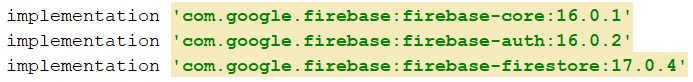
\includegraphics[width=0.5\textwidth]{images/firebase_gradle}
	\caption{A Firebase függőségei\label{fig:ALAP:sm2}}
\end{wrapfigure}

Adatbázisnak és az autentikáció menedzselésére Firebase-t használtam. Mielőtt bármilyen funkcióját is használhatnám ennek az applikációfejlesztési platformnak, be kellett jelentkezzek a Google felhasználómmal, készítenem kellett egy projektet, majd ezt a projektet össze kellett kapcsolnom magával az applikációval amit fejleszteni szerettem volna. Van egy külön \(plugin\)%
\footnote{ %
	kiegészítés
}  %
 az \(Android Studio\)%
 \footnote{ %
 	fejlesztési környezet android applikációk számára
 }  %
-ban, melynek segítségével könnyedén létre lehet hozni a ezt kapcsolatot. Előtte azonban az applikáció Gradle állományába be kellett jelentsem a \(core\), \(auth\) és \(firestore\) modulokat, mint függőségeket.
 

 

\subsection{Autentikáció}

A web-es felületen engedélyeznem kellett az e-mail/jelszó bejelentkezést. Ugyanitt állítottam be, hogy biztonsági okokból maximum hány regisztrációt engedjen a rendszer óránként ugyanarról az IP címről, jelenleg ez 100. Regisztációkor generálódik egy egyedi felhasználói ID, ennek segítségével oldom meg, hogy minden felhasználó csak a saját adataihoz férjen hozzá. A bejelentkezés, regisztráció, jelszó visszaállító e-mail küldése műveleteket a FirebaseAuth \(singleton\)%
\footnote{ %
	egy tervezési minta, az adott osztályból egy és csak is egy objektumot lehet létrehozni
}  %
 osztály metódusaival oldottam meg.
 
 \begin{description}
 	\setlength{\itemsep}{0.04mm}
 	\item[createUserWithEmailAndPassword(email, jelszó)] -- kreál egy felhasználót az e-mail és jelszó karakterlánc paraméterek segítségével, majd sikeres válasz után be is jelentkezik
 	\item[signInWithEmailAndPassword(email, jelszó)] -- megpróbál bejelentkezni a megadott e-mail/jelszó kombinációval
 	\item[sendPasswordResetEmail(email)] -- küld egy jelszó visszaállító e-mailt a paraméterként megadott címre.
 \end{description}

Az aktiváviós e-mail küldéséhez a FirebaseUser osztály insztanciájának a sendEmailVerification() metódusát használtam.

\subsection{Kollekciók, Dokumentumok}

\begin{wrapfigure}{l}{0.6\linewidth}
	\centering
	\setlength{\abovecaptionskip}{0pt}
	\setlength{\belowcaptionskip}{0pt}
	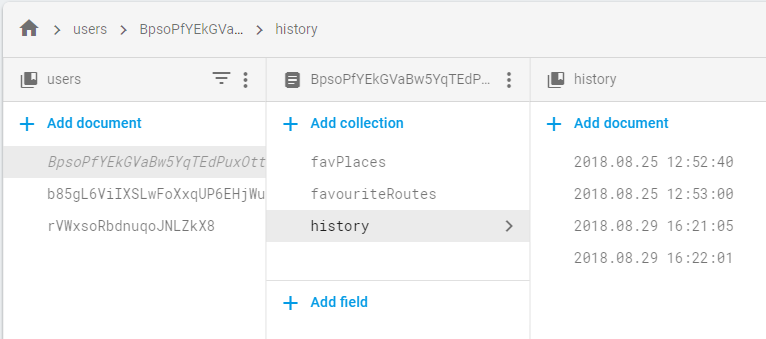
\includegraphics[width=0.6\textwidth]{images/firestore_colls}
	\caption{Firestore kollekciók\label{fig:ALAP:sm2}}
\end{wrapfigure}

A Firestore egy még Beta%
\footnote{ %
	még tesztelés alatt van
}  %
 verzióban levő no-sql, kulcs-érték párokra alapuló adatbázis, mely a Firebase platformon érhető el. Építőelemei a kollekciók és a dokumentumok, ezek váltakozva követik egymást, mivel egy kollekció csak dokumentumokat tartalmazhat, egy dokumentom viszont a kollekciók mellett adatokat (kulcs-érték párok) is tartalmazhat. 
 
 \begin{wrapfigure}{l}{0.6\textwidth}
 	\centering
 	\setlength{\abovecaptionskip}{0pt}
 	\setlength{\belowcaptionskip}{0pt}
 	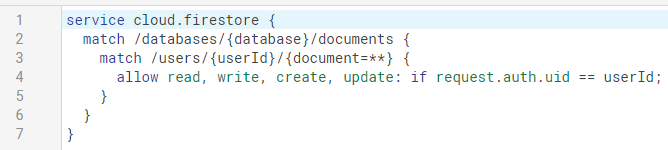
\includegraphics[width=0.6\textwidth]{images/firestore_rule}
 	\caption{Firestore szabály\label{fig:ALAP:sm2}}
 \end{wrapfigure}
 
Minden felhasználónak csak a saját dokumentumához van hozzáférése. Ezt egy úgynevezett szabály meghatározásával lehet elérni. Az adatbázis minden beérkező függvényhívást kiértékel a szabály alapján, és eldönti, hogy az adott kérésnek van-e elegendő jogosultsága. Amennyiben nincs, csak egy hibaüzenetet térít vissza.

 A GRoutes alkalmazás esetében a következőképpen építettem fel a struktúrát: vagy egy \(users\) kollekció, amely a felhasználókat tartalmazza. Minden felhasználói dokumentumnak az ID-ja megegyezik az UID%
\footnote{ %
	egyedi felhasználói ID, ami regisztrációkor generálódik
}  %
-val. A felhasználói dokumentumok a \(favPlaces\), \(favouriteRoutes\) és \(history\) kollekciókat tartalmazzák, melyek rendre megfelelnek a "kedvenc helyek", "kedvenc útvonalak" és "múltbeli útvonalak" fogalmaknak. Ezek a kollekciók tartalmazzák a különböző bejegyzéseknek (helyek, útvonalak) megfelelő dokumentumokat, melyek magukat az adatokat tartalmazzák. Az adatok sajátos entitás objektumok, melyeket a kódban, bizonyos szabályok alapján, de az én elképzelésem szerint hoztam létre. 


Egy út tartalmaz egy hely objektumokból álló tömböt a csomópontok számontartására, egy indexekből álló tömböt a csomópontok sorrendjének tárolására, valamint egy név mezőt.

Egy hely objektum tartalmaz egy-egy karakterlánc típusú név és cím mezőt, valamint egy GeoPoint objektumot, ami a hely főldrajzi szélességi és hosszúsági fokait tárolja.
 

%%%%%%%%%%%%%%%%%%%%%%%%%%%%%%%%%%%%%%%%%%%%%%%%%%%%%%%%%%%%%%%%%%%%%%%
\section{Osztályok}\label{sec:ALAP:adatelem}

\begin{figure}
	\centering
	\setlength{\abovecaptionskip}{-10pt}
	\setlength{\belowcaptionskip}{0pt}
	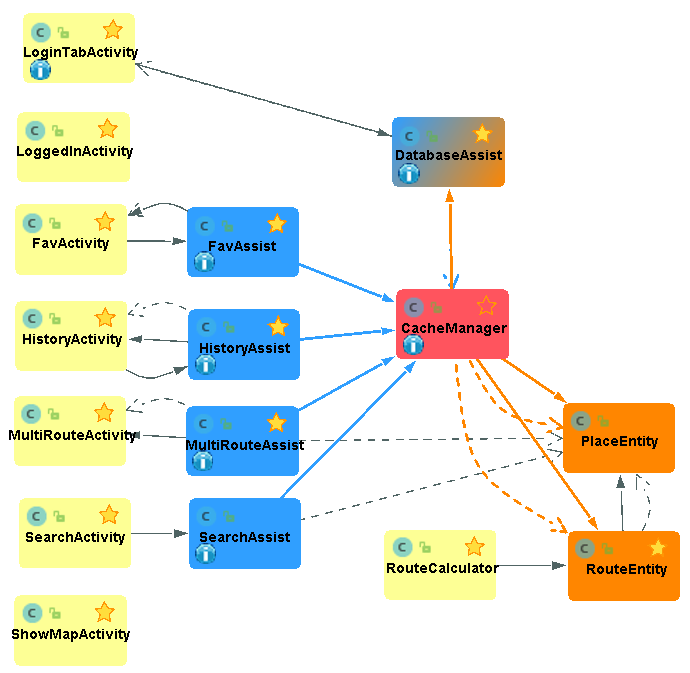
\includegraphics[width=1\textwidth]{images/class_diagram}
	\caption{Osztálydiagramm\label{fig:ALAP:sm2}}
\end{figure}

\subsection{Activity-k}\label{sec:ALAP:adatelem}

Egy android applikációban a UI%
\footnote{ %
	user interface - felhasználói felület
}  %
-t XML%
\footnote{ %
	Extensible Markup Language - Kiterjeszthető Jelölő Nyelv
}  %
állományok segítségével szerkeszthetjük meg, ezek azonban csak a külalakot adják meg. A háttérben végrehajtódó logikáért az Activity osztályok felelnek. A GRoutes alkalmazás különböző használati eseteihez más-más \(activity\) és XML állománypár tartozik.

\begin{description}
	\setlength{\itemsep}{0.04mm}
	\item[LoginTabActivity] -- ez a bejelentkezési felület, tehát ez fogad minket az alkalmazás indításakor. Itt történik az e-mail és a jelszó mezők validálása, formátum ellenőrzése a bejelentkezési próbálkozás előtt. Használja a DatabaseAssist autentikációval foglalkozó metódusait, majd a válasz visszaérkezése után a LoggedInActivity-hez navigál.
	\item[LoggedInActivity] -- ez a főmenü. Amint beléptünk ide, a háttérben betöltjük a felhasználó adatait (múltbeli keresések, kedvencek). Innen tudunk tovább navigálni a főbb menüpontokhoz.
	\item[FavActivity] --  ez a "Kedvencek" felület. Mivel itt már komplexebb műveleteket kell végrehajtani, ezért azokat egy segédosztályba csoportosítottam, egy köztes réteget létrehozva a UI és az adatbázissal foglalkozó osztály között.
	\item[HistoryActivity] -- ez a "múltbeli keresések" menüpont, rendelkezik segédosztállyal 
	\item[MultiRouteActivity] -- ez felel az útvonalak kirajzolásáért, rendelkezik segédosztállyal 
	\item[SearchActivity] -- ez a keresés menüpont, rendelkezik segédosztállyal 
	\item[ShowMapActivity] -- a helyek megjelenítéséért felel
\end{description}

\subsection{Assist osztályok}\label{sec:ALAP:adatelem}

Általánosan, az alábbi segédosztályok végzik el a különböző Activity-k feladatait. Továbbá ők vannak kapcsolatban a CacheManager osztállyal, amely az adatok frissen tartásáért felel.

\begin{description}
	\setlength{\itemsep}{0.04mm}
	\item[FavAssist] -- feltölti adatokkal a "Kedvencek" felületet, dinamikusan beágyazza az XML-be a bejegyzéseket, továbbítja az activity módosítási, törlési szándékait a CacheManagernek
	\item[HistoryAssist] -- a FavAssist osztályhoz hasonló feladatokat végez el a HistoryActivity-nek. Egy múltbeli keresés kedvencekhez való hozzáadását is lemenedzseli
	\item[MultiRoutAssist] -- lekéri a csomópontok közti útvonalat a DirectionApi segítségével, majd kirajzolja a tervezett útvonalat a Polyline%
	\footnote{ %
		vonallánc
	}  %
 osztály használatával. A navigálásért is felel.
	\item[SearchAssist] -- feldolgozza a keresési címeket, majd a megfelelő adatstruktúrát lekommunikálja a CacheManager-nek
\end{description}

\subsection{Általános segédosztályok}\label{sec:ALAP:adatelem}

A fontosabb általános műveletek végrehajtására létrehoztam néhány Singleton mintára készült segédosztályt.

\begin{description}
	\setlength{\itemsep}{0.04mm}
	\item[DatabaseAssist] -- ez felel mindennemű Firebase-el kapcsolatos kommunikációért. Feladatai közé tartozik a regisztráció, bejelentkezés, az ezekkel kapcsolatos e-mail küldések, valamint a CRUD operációk elvégzése.
	\item[CacheManager] -- a köztopnti adatmenedzselő osztály. Ő tölti be, aktualizálja, szolgálja ki a segédosztályokat az adatokkal, továbbítja kéréseiket a DatabaseAssist-nak. A LoginTabActivity kivételével csak ő áll kapcsolatban a DatabaseAssist segédosztállyal.
	\item[RouteCalculator] -- az optimális útvonal meghatározásáért felel (az utazó ügynök problémájának megoldása)\cite{pyconc}
\end{description}

\subsection{Entitás osztályok}\label{sec:ALAP:adatelem}

Az alkalmazás két nagyon fontos logikai struktúrát használ: helyek és útvonalak. Ezekkel több műveletet is kell végezni, mint például átalakítások, keresések, bizonyos paraméter alapján történő módosítások. Ezért számukra létrehoztam egy-egy entitás osztályt. 

A Firestore-ba való egyszerű mentés érdekében bizonyos kritériumoknak meg kell felelniük: rendelkezniük kell egy paraméter nélküli publikus konstruktorral, valamint az elmenteni kívánt attríbútumoknak publikus \(getter\) metódusokkal. Ezért azoknak az attribútumoknak a \(getter\) metódusait, amelyeket nem kívántam elmenteni, átneveztem úgy, hogy a \(ret%
\footnote{ %
	return - visszatérít
}  %
-\) prefixet használtam.

\begin{description}
	\setlength{\itemsep}{0.04mm}
	\item[PlaceEntity] -- három attribútuma van: egy String típusú név, egy GeoPoint típusú (magába foglalja a földrajzi szélességi és hosszúsági fokokat) helyszín és egy String típusú cím
	\item[RouteEntity] -- négy attribútuma van: egy String típusú ID (az adatbázisban történő azonosításra), egy String típusú név, egy egész számokból álló ArrayList típusú sorrend (a csomópontok bejárási sorrendjének tárolására) valamint egy helszínekből álló ArrayList típusú csomópont (csomópontok tárolása)
\end{description}



%%%%%%%%%%%%%%%%%%%%%%%%%%%%%%%%%%%%%%%%%%%%%%%%%%%%%%%%%%%%%%%%%%%%%%%
\section{Felmerülő problémák}\label{sec:ALAP:adatelem}


\subsection{Aszinkron függvényhívások}\label{sec:ALAP:adatelem}

Több olyan használati eset van, amikor egy bizonyos metódus az interneten keresztül kommunikál egy szerverrel. Ez mindig okozhat problémákat, de a szinkronhívásokat kivételkezeléssel egyszerúen meg lehet oldani. Több esetben, mint például a bejelentkezéskor vagy az adatok lekérdezésekor, a program nem vár a válaszra, hanem tovább végzi a következő műveleteket. Ez olyan helyzetekhez vezethet, hogy megnyitunk egy felületet és még nincsenek beöltve az adataink. 

Ezt a problémát úgy oldottam meg, hogy a DatabaseAssist osztály fog utólag jelezni annak az osztálynak ahonnan a kérés érkezett, amint választ kapott.


\subsection{Adatok aktualizálása az activity-k között}\label{sec:ALAP:adatelem}

Mivel az applikáció több különböző pontján van lehetőség az adatok hozzáadására, módosítására, törlésére, ezért fontos, hogy mindig, mindenhol a legfrissebb adatok birtokában legyünk.

Ezért vezettem be a CacheManager osztályt. Ez nem csak tárolja az aktuális adatokat, hanem az első lekérdezés kivételével, minden adatbázisműveletet lokálisan is elvégez, így a felhasználónak nem kell várnia, hogy a "múltbeli keresések" menüpont alatt megjelenjen a friss keresés, mivel azonnal hozzá lesz adva. Ellenkező esetben meg kéne várni, míg elmentjük az adatokat, majd lekérdezzük őket.

\subsection{Koordináta osztályok}

Egy földrajzi koordináta nem egy bonyolult adatszerkezet: tartalmaz egy földrajzi szélességi fokot, valamint egy hosszúsági fokot. Mégis három különböző osztályra volt szükség a reprezentálásához. 

\begin{description}
	\setlength{\itemsep}{0.04mm}
	\item[GeoPoint] -- a Firestore egyik beépített adattípusa, így az adatbázis miatt, az egyszerű tárolás, valamint CRUD műveletekkel való kompatibilitás miatt szükség volt ennek használatára.
	\item[com.google.android.gms.maps.model.LatLng] -- a GoogleMap osztály használja. Ha egy \textit{Marker}-t szeretnénk egy térkép \textit{activity}-ben használni, akkor egy ilyen objektumot kell paraméterként átadjunk.
	\item[com.google.maps.model.LatLng] -- a Direction API, valamint a Distance Matrix API metódusaiban, paraméterként használt típus.
\end{description}

A \textit{Java} nyelvben nincs lehetőség egy importált osztály elnevezésére úgy, mint például \textit{Python}-ban. Ez azt eredményezte, hogy minden \textit{LatLng} típusú objektum létrehozásakor explicit meg kellett adni az egész csomag (\textit{package}) importálási ösvényét, mivel a két osztály neve megegyezik, és ez ambiguitást eredményez a \textit{compiler} számára.



%!TEX root = GRoutes.tex
%%%%%%%%%%%%%%%%%%%%%%%%%%%%%%%%%%%%%%%%%%%%%%%%%%%%%%%%%%%%%%%%%%%%%%%
\chapter{Következtetések}\label{ch:ALAP}
%%%%%%%%%%%%%%%%%%%%%%%%%%%%%%%%%%%%%%%%%%%%%%%%%%%%%%%%%%%%%%%%%%%%%%%

A tudomány jelenlegi állása szerint nem létezik olyan algoritmus, amely polinomiális komplexitással rendelkezik, és meg tudja oldani egzakt módon az utazó ügynök problémáját. A gyakorlati felhasználói esetekben, azonban nem is biztos, hogy mindig erre van szükség. Az alkalmazásokat adaptívnak kell készítenünk, és a felhasználónak meg kell adjuk a lehetőséget, hogy a saját felhasználási igényeihez mérten testre tudja szabni azokat. Így tehát ez a projekt egy ötletet adhat azoknak, akik bizonyos helyzetekben egy, míg bizonyos helyzetekben más megoldási módszereket alkalmaznának. Az egzakt algoritmusoknál a bemenő adatok növekedésével párhuzamosan, a végrehajtási idő exponenciálisan növekszik. A mohó algoritmusok ezzel ellentétben nagy mennyiségű bemeneti adatra is nagyon gyorsan képesek meghatározni egy megoldást, azonban az nem biztos, hogy ez az optimális megoldás lesz. Azt viszont csak a felhasználó tudja, hogy milyen célra, vagy mikor milyen célra szeretné használni az alkalmazást. Így tehát a döntés lehetőségét az ő kezébe helyeztük.

A későbbiekben szeretném az alkalmazást egy újabb funkcionalitással, valamint platformmal kibővíteni. A csoportok menüpont alatt lehetőség nyílik arra, hogy a felhasználók egymásnak tervezzenek útvonalakat, megosszák ezeket, valamint arra is, hogy cégen belül az irodából lehessen frissíteni a terepen dolgozó kolléga további állomásait. Ehhez szeretnék majd egy web-es felületet is készíteni, hogy az irodából egyszerűbben, kényelmesebben lehessen nagyobb mennyiségű adattal dolgozni. A személyreszabhatóság növelésének érdekében több kritérium megadására is lehetőség lesz, mint például az adott helyszínekhez köthető nyitvatartási időintervallum\cite{gt_problem}\cite{gt_and_appl}\cite{gt_alg_india}\cite{comp_tsp}





{ \renewcommand{\baselinestretch}{0.8}\normalsize %
	\setlength{\itemsep}{-2.4mm}
	\setlength{\bibspacing}{0.67\baselineskip}
	\bibliographystyle{abbrvnat_hu}
	\bibliography{dolgozat}
}
\end{document}
